\documentclass[tikz,border=6pt]{standalone}
\usepackage{amsmath,amssymb}
\usepackage{xcolor}
\definecolor{accent}{HTML}{A13D2C}
\definecolor{accent2}{HTML}{2B5F6B}
\definecolor{muted}{HTML}{5A564F}
\definecolor{panel}{HTML}{F8F6F0}
\definecolor{linecol}{HTML}{D8D2C4}
\definecolor{astroblue}{HTML}{1B4F72}
\definecolor{ink}{HTML}{1E1C1A}
\usetikzlibrary{calc,arrows.meta,angles,quotes}
\usepackage[T1]{fontenc}\usepackage{newpxtext,newpxmath}  % same fonts as the notes
\begin{document}
% Polar coordinates in the orbit plane: X along the node direction n-hat, Y in the plane, Z out of
% the page along L. The body at distance r and angle phi, with the unit vectors r-hat and phi-hat.
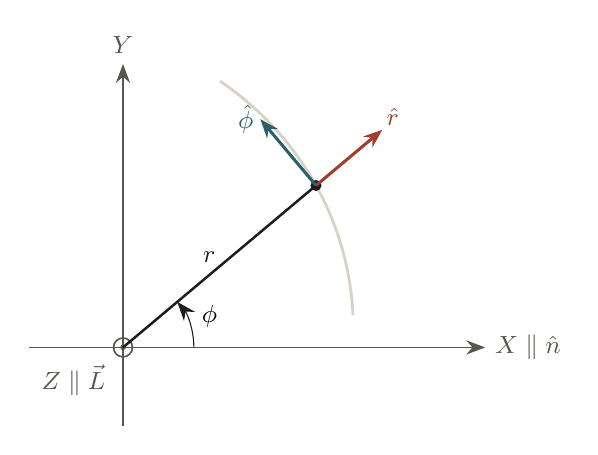
\begin{tikzpicture}[font=\small, >={Stealth[length=2.4mm]}]
  \def\ph{40}\def\r{3.2}
  \draw[muted, ->, line width=0.6pt] (-1.2,0) -- (4.6,0) node[right] {$X\parallel\hat n$};
  \draw[muted, ->, line width=0.6pt] (0,-1.0) -- (0,3.6) node[above] {$Y$};
  \draw[muted, line width=0.6pt] (0,0) circle (0.12); \fill[muted] (0,0) circle (0.035);
  \node[muted, anchor=north east] at (-0.1,-0.1) {$Z\parallel\vec L$};
  % a piece of the orbit through the body
  \draw[linecol, line width=1pt, domain=\ph-32:\ph+30, samples=40] plot (\x:{\r*1.125/(1+0.25*cos(\x-\ph+60))});
  \coordinate (O) at (0,0); \coordinate (P) at (\ph:\r); \coordinate (X) at (1,0);
  \draw[ink, line width=0.9pt] (O) -- node[above left, inner sep=1pt] {$r$} (P);
  \fill[ink] (P) circle (0.07);
  \pic[draw=ink, ->, "$\phi$", angle radius=0.9cm, angle eccentricity=1.3] {angle = X--O--P};
  \draw[accent, ->, line width=1.1pt] (P) -- ++(\ph:1.1) node[anchor=south west, inner sep=1pt] {$\hat r$};
  \draw[accent2, ->, line width=1.1pt] (P) -- ++(\ph+90:1.1) node[anchor=east, inner sep=2pt] {$\hat\phi$};
\end{tikzpicture}
\end{document}
